\documentclass[table, 12pt]{article}
\usepackage{graphicx}
\usepackage[T1]{fontenc}
\usepackage{tocloft}
\usepackage{todonotes}
\usepackage{caption}
\usepackage{hyperref}
\usepackage{booktabs}
\usepackage{listings}
\usepackage{pdfpages}
\usepackage{pdflscape}
\usepackage{textpos}
\usepackage{scrhack}
\usepackage{xcolor}
\usepackage{float}
\usepackage{longtable}
\usepackage{enumitem}
\usepackage{tasks}
\usepackage{tabularx}
\usepackage{titlesec}
\usepackage{listing}
\usepackage{graphicx}


\titleformat{\paragraph}
{\normalfont\normalsize\bfseries}{\theparagraph}{1em}{}
\titlespacing*{\paragraph}
{0pt}{3.25ex plus 1ex minus .2ex}{1.5ex plus .2ex}
\begin{document}
\begin{titlepage}
    \centering
    {\scshape\large AY 2020/2021 \par}
    \vfill
    
\includegraphics[width=100pt]{assets/logo-polimi-new}\par\vspace{1cm}
    {\scshape\LARGE Politecnico di Milano \par}
    \vspace{1.5cm}
    {\huge\bfseries Implementation Document \par}
    \vspace{2cm}
    {\Large {Luca Pirovano\quad Nicolò Sonnino}\par}
    \vfill
    {\large Professor\par
        Matteo \textsc{Rossi}}
    \vfill
    {\large \textbf{Version 1.0} \\ \today \par}
\end{titlepage}
\hypersetup{%
    pdfborder = {0 0 0}
}
\thispagestyle{plain}
\pagenumbering{gobble}
\mbox{}
\newpage
\pagenumbering{roman}
\tableofcontents
\newpage
\pagenumbering{arabic}

\section{Introduction}
\subsection{Purpose}
This document aims to describe how the implementation and integration testing took place.
Implementation is the last step of the CLup application development cycle.

Testing, instead, means check that the critical parts of the application works in a correct way, as described in the DD document.

The code and the releases can be find on the official CLup repository hosted on GitHub, reachable at this link:\\ \href{https://github.com/PiroX4256/SE2-Piemonti-Pirovano-Sonnino}{https://github.com/PiroX4256/SE2-Piemonti-Pirovano-Sonnino}.

\subsection{Definitions, Acronyms, Abbreviations}
\subsubsection{Definitions}
\subsubsection{Acronyms}
\begin{itemize}
    \item \textbf{DD:} Design Document
    \item \textbf{RASD:} Requirements Analysis and Specification Document
    \item \textbf{S2B:} Software To Be
    \item \textbf{DTO:} Data Transfer Object, represents a link between the user input and a Java Object.
\end{itemize}
\subsubsection{Abbreviations}
\subsection{Revision history}

\newpage
\section{Development}
\subsection{Implemented Functionalities}
With respect to the RASD and DD documents, we decided to implement the following functions:
\begin{itemize}
    \item \textbf{Sign Up}
    \item \textbf{ASAP: As Soon As Possible}
    \item \textbf{Hand out tickets on spot}
\end{itemize}
For more details regarding the specific functionalities, you are invited to read the RASD document, which contains a very detailed description of them.

We chooses to implement these functionalities in order to simulate a Module 1 product purchase. In fact, we remind that the application is divided into three modules; the first one is also called \textit{MVP}, and contains the basic functionalities of CLup, the second one contains the \textit{Book a Visit} feature and the last one includes the custom deploy on organization's servers.

In a real-world scenario, the most used module would be of course the first one (due to its simplicity), so that we decided to focus on it.

\subsection{Adopted Development Frameworks}
As we said in our DD, the application should follow a four-tier architecture, with a fully REST interface and a lot of client scripting. Finally, we decided to adopt the Model-View-Controller pattern, which is one of the most used in distributed applications.

In the following pages you will find a list of adopted frameworks and technologies in order to accomplish to this requirements.

\subsubsection{Programming languages}
For sake of standards and application speed we decided to use the Java\texttrademark  Programming Language, which is one of the most used languages in web and distributed applications.

Of course, there are some pros and cons about using this type of language:
\\\begin{itemize}
    \item \textbf{Pros:}
          \begin{itemize}
              \item[+] Speed: of course, since it is a compiled language, Java permits to have very good performances on these elaborations;
              \item[+] Standard: as shown in figure \ref{languages_comparison}, Java is the \textit{De Facto standard} in enterprise web development and represents a very good solution for portable applications;
              \item[+] Stability: Java is a mature language that has immensely evolved over the years. Hence it’s more stable and predictable.
              \item[+] Object-Oriented: The object-oriented nature of Java allows developers to create modular programs and write reusable codes. This saves lots of efforts and time, improving the productivity of the development process.
              \item[+] Well-documented
          \end{itemize}
    \item \textbf{Cons:}
          \begin{itemize}
              \item High verbosity: with respect to other programming languages (such as Python), Java contains a more verbose and less-readable syntax.
              \item High memory consumption: since Java Programs run on top of Java Virtual Machine, it consumes more memory.
          \end{itemize}
\end{itemize}

For the client-side scripting, we decided to adopt JavaScript\texttrademark  for the web app, and Flutter with Dart\texttrademark  languages for the mobile app.

JavaScript is a text-based programming language used both on the client-side and server-side that allows to make web pages interactive. Where HTML and CSS are languages that give structure and style to web pages, JavaScript gives web pages interactive elements that engage a user.

Flutter, instead, is an open-source UI software development kit created by Google. It is mostly used to develop applications for Android and iOS.

\begin{figure}[H]
    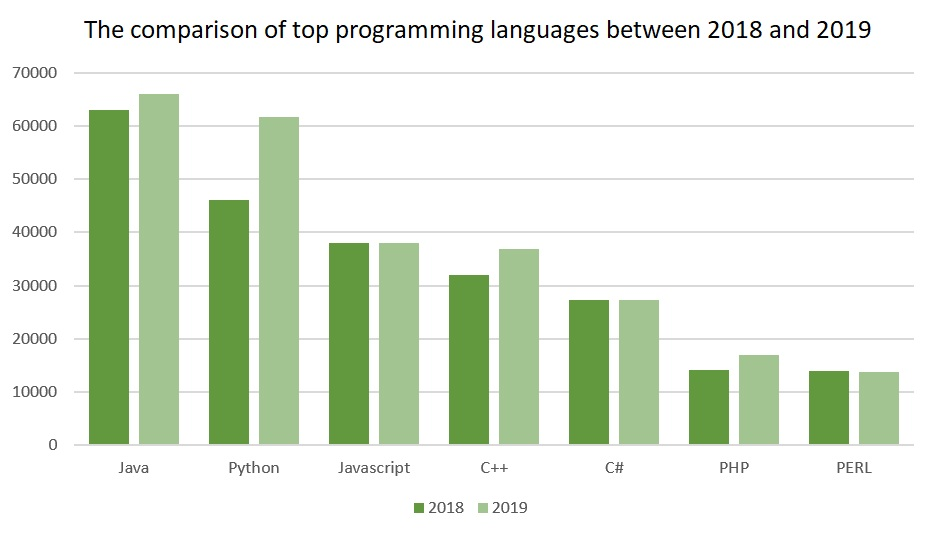
\includegraphics[width=\textwidth]{assets/graph-18-19-languages.jpg}
    \caption{Web Programming languages usage (2018 vs 2019)}
    \label{languages_comparison}
\end{figure}

\begin{figure}[H]
    
\includegraphics[width=\textwidth]{assets/client-side-scripting.png}
    \caption{Client-side technologies}
\end{figure}

\subsection{Java Frameworks}
\subsubsection{Spring}
In order to accomplish the S2B requirements, we decided to adopt the Spring development framework.

Spring is an open source framework, used for RESTful Java application development. It's built on top of the Java Enterprise Edition (JEE) and represents an efficient and modern alternative to the classic Enterprise Java Bean (EJB) model.

Of course, using a framework means works on a solid base, which is well tested and documented. In fact, Spring contains a proper paradigm in order to build web services on its API.

\begin{figure}
    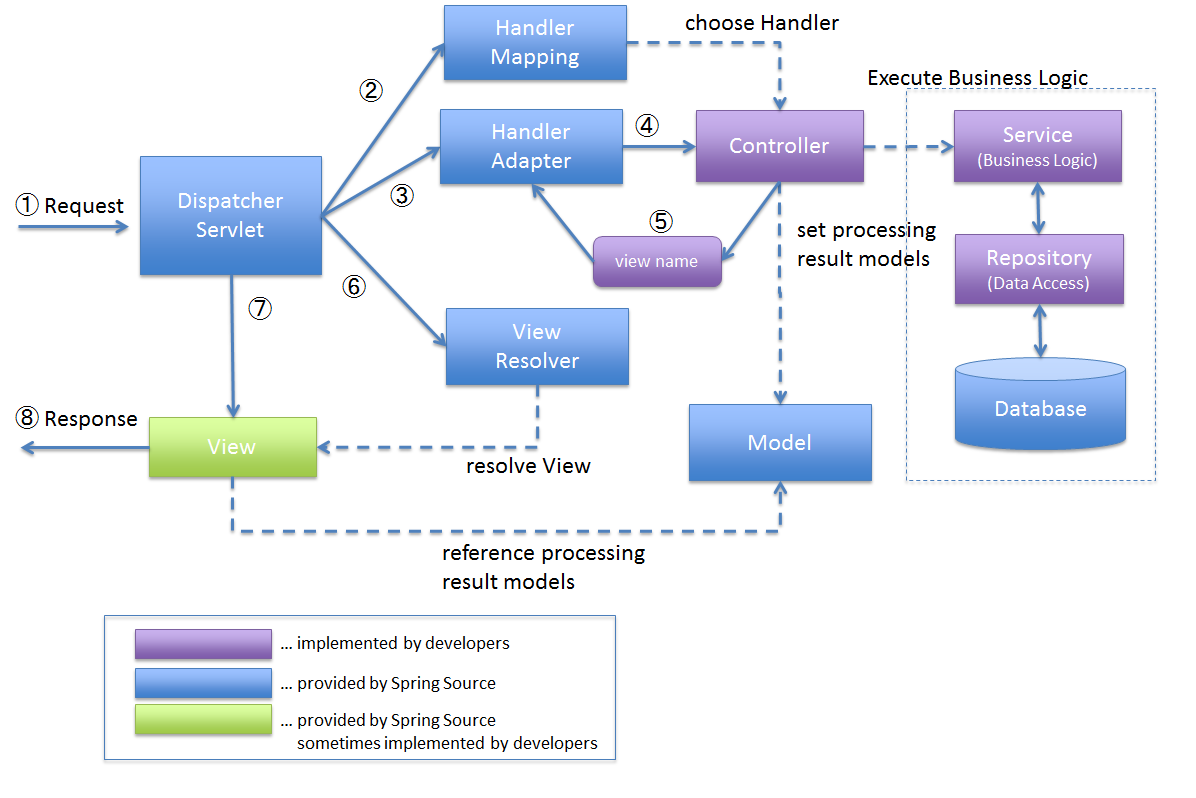
\includegraphics[width=\textwidth]{assets/SpringArchitecture.png}
    \caption{Spring Framework architecture}
    \label{spring_architecture}
\end{figure}

As shown in figure \ref{spring_architecture}, the architecture of Spring is very simple and easy-to-use.

In fact, it is composed by:
\begin{itemize}
    \item \textbf{Dispatcher Servlet:} its job is to route all the incoming requests to the correct Spring controller, which is properly mapped with an appropriate annotation. This is done through the severals components of Spring, which are HandlerMapping, HandlerAdapter and ViewResorver.
    \item \textbf{Controller:} the controller acts as an interface between the user and the services. It catches the requests coming from the dispatcher and makes actions relying on what user passed to it.
    \item \textbf{Model:} it contains the application logic about the transfer objects (also called DTO) which maps a user input (which is encoded in JSON format) and a Java object. The DTOs can also be used in the opposite direction (server to client), so they are encoded in JSON format and then sent to the client.
    \item \textbf{Services:} they act as an intermediate between the entities (database objects) and the controller, containing some useful methods in order to manipulate data sent by controllers.
    \item \textbf{Repositories:} they are interfaces that contains the query methods in order to fetch data from database. They are managed from Spring engine and it suffices to specify what to retrieve in order to get a response object from the DBMS.
    \item \textbf{Entities:} they represent database objects. They are declared with @Entity annotation, which maps the object to a database table (or set of them). Inside an entity object it is possible to specify constraints and foreign references through proper annotations.
\end{itemize}

\subsubsection{Spring Data JPA}
Spring Data JPA, part of the larger Spring Data family, makes it easy to easily implement JPA based repositories. This module deals with enhanced support for JPA based data access layers. It makes it easier to build Spring-powered applications that use data access technologies.

Spring Data JPA aims to significantly improve the implementation of data access layers by reducing the effort to the amount that’s actually needed.

In fact, through services and repositories, interfacing with the database becomes very simple. Useless to say that, furthermore, the security of the queries from SQL injection is high, because it is totally managed by Spring.

\subsubsection{Spring Security}
\subsubsection{Spring Social}

\subsection{Other Frameworks}
\subsubsection{Vue.js}
\subsubsection{jQuery}
\todo[]{Insert qr code library}

\newpage
\section{Source Code}

\newpage
\section{Testing}

\newpage
\section{Installation Instructions}
\end{document}